\documentclass[12pt]{article}
%Uncomment next line if AMS fonts required
%\usepackage{iopams}
\usepackage{graphicx}
\usepackage{hyperref}   % to set up hyperlinks
\hypersetup{
	colorlinks=true,
	linkcolor=blue,
	citecolor=blue,
	urlcolor=blue,
}

\begin{document}

%%\note{A novel passive
%%ferrofluid check (one-way) valve}

\title{Pumping Ferrofluid With Only Liquid}

\maketitle

%%% first author
\author{Robert L. Read}

\begin{abstract}

  Currently this is very preliminary. This is an attempt to design a pump that can efficiently pump ferrofluid with no moving parts
  except the ferrofluid and two blobs of an immiscible, incompressible fluid, such as water.
  Eliminating moving parts allows miniaturization and potentially fabrication as a chip.
  A miniature pump could be used for cooling a chip and for ``lab on a chip'' applications.
  The proposed design uses two permanent magnets and seven controllable electromagnets.
  The design was developed from considering the minimal topological connection of fixed chambers.
  It has four distinct phases, each phase having a distinct magnetic configuration.
\end{abstract}

%
% Uncomment for keywords
\vspace{2pc}
\noindent{\it Keywords}: ferrofluid pump

% Uncomment if a separate title page is required
%\maketitle
%
% For two-column output uncomment the next line and choose [10pt] rather than [12pt] in the \documentclass declaration
%\ioptwocol
%


%%%%%%%%%%%%%%%%%%%%%%%%%%%%%%%%%%%%%%%%%%%%%%%%%%%%%%%%%%%%%%%%%%%%%%
\section{Introduction}

Ferrofluid can be manipulated by electronically controlled magnetic
fields to exert force on fluids\cite{torres2014recent,kole2021engineering,ozbey2015modeling}.
This makes it possible to build pneumatic or hydraulic
devices, perhaps on very small scales,
such as a single chip\cite{yamahata2003ferrofluid,hatch2001ferrofluidic}, to
miniaturize fluid handling.
This has been proposed for biomedical purposes\cite{michelson2019novel}
that would use water or body fluids,
although this paper reports only on experiments done with air.
Miniature pumps and valves could be used to make a “lab on a chip” (LOC) or
even to heat or cool different chip areas.

%%%%%%%%%%%%%%%%%%%%%%%%%%%%%%%%%%%%%%%%%%%%%%%%%%%%%%%%%%%%%%%%%%%%%%
\section{Related Research}

A number of papers report on ferrofluid pumps, focusing in particular
on micropump and lab-on-a-chip applications\cite{ozbey2015modeling,hsu2018biocompatible}.
Many of these papers use
a version of mechanical valve not based on passive
ferrofluid, even though they move a ferrofluid bolus
with a magnetic field.
For example,
a corrugated silicone micro valve\cite{yamahata2003ferrofluid,yamahata2005plastic}
has been reported.
Other researchers use active valves, which require synchronization with
the ferrofluid plug to form a pump,
such as \cite{menz2000fluidic}, which
describes an active {\em T-Valve} with a moving ferrofluid plug, and
\cite{ando2009ferrofluidic} describes a complete fluid pump with valves
that use
active control of a ferrofluid bolus.
At least two additional kinds of active valves, a {\em well valve} and
{\em Y-valve}, have
been described\cite{hartshorne2004ferrofluid}.
Active control is possible because the
action of the plunger or bolus may be synchronized with the opening and closing
of the valves.
Nonetheless a passive valve would be simpler and less
expensive, and would not require knowledge of the timing of the
plunger.

An interesting functional micropump in which the
moving ferrofluid bolus merges with a fixed ferrofluid valve and then
separates on each pumping cycle has been described\cite{hatch2001ferrofluidic}.

An interesting devices induces a flow directly in ferrofluid
with no moving parts,
presumable based on the rotation of clumps of ferrofluid
\cite{mao2011direct}.

\section{The Idea}

There is no known way to directly move a mass of ferrfluid which is immersed in
ferrofluid.
The idea of moving a ferrofluid plug or bolus which is bouneded by air or water
via electromagnets turned on or off is well known. A slight inversion of this
idea is to use two boluses to trap a blob of water. The water thus remains
a separator. In the diagrams below it is represented as a ``W'',
and the ferrofluid as an ``F''.
The separator allows us to move the bolus slightly.
In order to create a pump, we need to recycle this separator, rather than
moving it once, as in a piston.

If we combine this with the idea of a moving bolus ``picking up'' some ferrofluid
and then dropping some of that ferrofluid, we can have a two circulating water blobs
and two circulating ferrofluid plugs. One ferrofluid plug, which is moving from the
inlet to the outlet, is larger.
The other plug is smaller, and merely separating the water plugs as it is returned.

If we reduce this to a minimal configuration, we have a circle of seven regions
of equal size. The inlet and the outlet prevent the water blobs from escaping by
having permanent magnets in place. The water blobs can never displace these
locks, represented by ``L'' in our diaggram. The inlet of the pump has an
inexhaustible supply of ferrofluid represented as a source (``S''). The
outlet is represented as a drain ``D''.

The water plugs must always be kept separated by ferrofluid plugs. However,
these plugs can pull fluid from the source and push it into the drain if
so driven by the changing magnets in the seven dynamic regions.
By cycling through four configurations as depicted, we can move ferrofluid
from the source to the drain.




\begin{figure}
\centerline{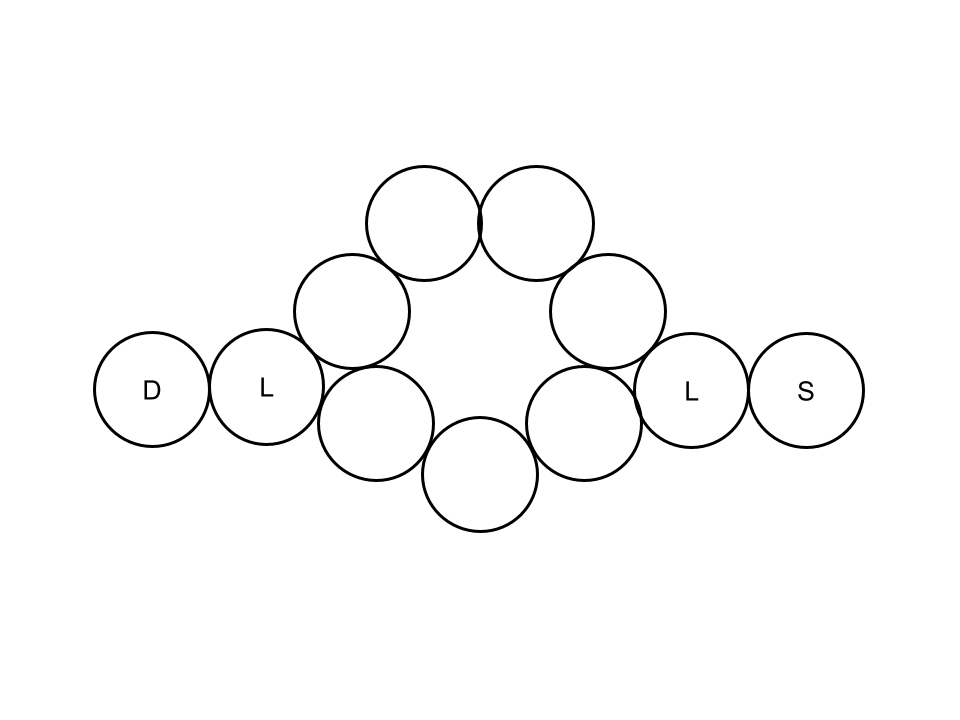
\includegraphics[width=5in]{images/Ferrofluid Pump.png}}
\caption{The Pump Schematic}
\label{fig_pumpschematic}
\end{figure}

\begin{figure}
\centerline{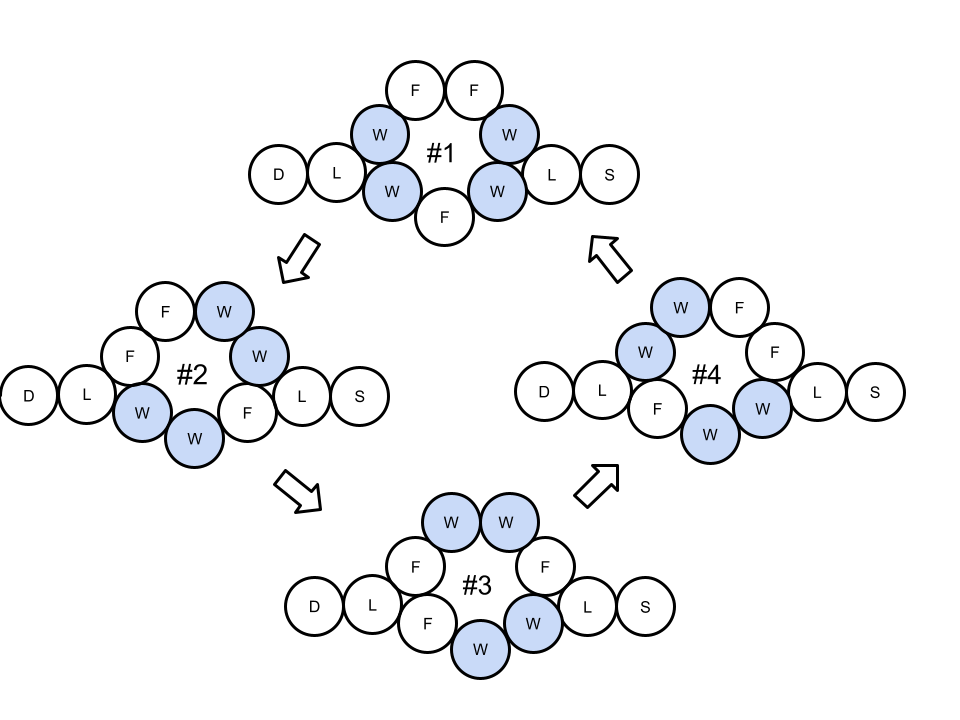
\includegraphics[width=5in]{images/PumpPhases.png}}
\caption{The Pump Schematic}
\label{fig_pumpschematic}
\end{figure}

\section{A Simple Test Apparatus}

It is easy to source permanent magnets and difficult to source electomagnets with
the precise shapes neede for this project.
A test apparatus using only permanent magnets moved by hand to match the 4-stroke cylce
of the pump should allow us to test the hypothesis that this pump will work and measure
flow on a per-cycle basis.
This approach will postpone the need to develop the electromanets.

We therefore propose to make 3D printed apparatus that has cages for permanent magnets
which can be moved into the pump ring and out of the pump ring to simulated turning
an elctromagnet on and off.
These cages are necessary because strong permanent magnets tend to want to fly into
each other and must be carefully constrained.
We believe we can furthermore make handles which we can glue to the magnets with
hot-melt glue to make the motion of the magnets easier to effect.
We suspect that the magnest will stay in place when in the ring,
and have to held when out of the ring, which may require three hands or
some dextrous holding.

\section{A Separate Test}

The idea presented in the paper assumes that a bolus of water which is trapped
between two boluses of ferrofluid will remain coherent. That is, it will
resist the intrusion of ``fingers'' or ferrofluid into the bolus of water.
For exmample, if a thin finger of ferrofluid reached into the water and
reached the other side, the ferrofluid could flow through the water by means
of this channel, and the moving boluses of water might not force the
ferrofluid to move in the way that would make this invention functional.

We can test this with a simpler apparatus.
Let us take a clear tube of acrylic and two strong permanent magnets.
Adhere the two magnets with the same polarity rather close to each other,
say 2 inches apart.
Close one end of the tube and mount it vertically.
Fill the tube with ferrofluid to just above the lower magnet.
Then fill the tube with water to just below the higher magnet.
Then fill the rest of the tube with ferrofluid.

My hypothesis is that the water will remain a coherent mass without
instrusions of ferrofluid. If we open the ends of the tube, we will
be able to slide out two magnets in relation to the tube, moving the
bolus with it.

I believe the reason the intrusions do not occur is what
Joe Herschberge has named ``magnetic buoyancy''. An intrusion
would increase potential energy, not because of the ferrofluid
in between the two magnets, but because it for a displacement of
water into the ferrofluid which is in a strong field.
That displacement would increase the potential energcy, and
therefore a force which we name {\em magnetic buoyancy} opposes it.

\subsection{A Way To Test it Simply}

Lawrence Kincheloe has provided this observation about testing this easily:


The 2d Ferro fluid pump could be easily executed with sheets of acrylic to form a fluid chamber. An external turntable with magnets attached could be used to test the idea, as displayed in the infographic.

\section{Motivation}

Lawrence Kincheloe suggested this approach:

Ferro fluids could be used for vein massages and pumping by direct injection into the veins. This is predicated on a biocompatible ferro fluid where the lipid shell and nano scale ferride can be adsorbed by the body and act like an iron supplement. The direction of an external magnetic field will direct the ferro fluid to a particular location and could allow for mechanical agitation, and a pumping action using a rhythmic compression and expansion of plasma displacement within the veins.

\section{Conclusions}

\section{TODO}

Study this: \url{http://citeseerx.ist.psu.edu/viewdoc/download?doi=10.1.1.719.4343&rep=rep1&type=pdf}

\section{Acknowledgements}

This paper was an outgrowth the the Passive Ferrrofluid Check Valve (PFCV) \cite{stuckeynovel}
reported by Veronica Stuckey and Robert L. Read. Veronica Stuckery 3D printed
some of the apparatus.

\section*{References}

\bibliographystyle{unsrt}
% Here's where you specify the bibliography database file.
% The full file name of the bibliography database for this
% article is asme2e.bib. The name for your database is up
% to you.
\bibliography{ffcv}

\end{document}
